% Estas slides tienen que abrirse con el programa pdfpc que soporta videos embebidos
% el comando es: pdfpc -g slides.pdf
% para los videos se requiere ubuntu-restricted-extras
% para la bibliografía se requiere biber y configurar texstudio

%\documentclass[compress,handout]{beamer}
\documentclass[aspectratio=169,compress]{beamer}

% add beamer preamble
% Theme customization
\setbeamertemplate{itemize item}[rectangle] % configure itemize
\setbeamertemplate{itemize subitem}[circle] % configure itemize
\setbeamertemplate{itemize subsubitem}[triangle] % configure itemize
\setbeamertemplate{navigation symbols}{} % remover simbolos de navegacion de las slides
\usefonttheme[onlymath]{serif} % simbolos matematicos en serif (Como es en latex original)
\setbeamersize{text margin left=3mm,text margin right=3mm} 

\setbeamertemplate{blocks}[rounded] % blocks corners rounded
\setbeamercolor{block body}{bg=blue!12,fg=black} % color of blocks
\setbeamertemplate{caption}{\raggedright\insertcaption\par} % elimina la palabra "Figura" del caption

\usepackage[overridenote]{pdfpc} % requires to download manually pdfpc.sty package from https://www.ctan.org/pkg/pdfpc

% add latex preamble
% para la bibliografía se requiere biber y configurar texstudio

% Latex packages
\usepackage[utf8]{inputenc}
\usepackage[T1]{fontenc} % para copiar acentos en español del pdf y permite acentos en las notas
\usepackage[spanish]{babel}
\usepackage[per-mode = symbol]{siunitx} % para manejar las unidades
\usepackage{multimedia} % to add videos with \movie command
\usepackage{multirow}
\usepackage{graphicx}
\usepackage{xcolor}
\usepackage{amsmath} % bmatrix
\usepackage[makeroom]{cancel} % \cancel to cancel terms in math equations
\renewcommand{\CancelColor}{\color{red}} % set red color for \cancel command
\usepackage[caption=false]{subfig} % caption = false elimina la palabra "Figura" del caption
\usepackage{import} % para el comando import (se usa para pdf_tex)
\captionsetup[subfigure]{labelformat=empty} % remover el indice del caption de la subfigura
\usepackage{booktabs} % \toprule \midrule \bottomrule
\usepackage[backend=biber]{biblatex} % set biber to format references. Must configure Biber in Texstudio
\usepackage{csquotes} % to remove warning triggered by biblatex and babel
\usepackage{algorithm} % to put captions to the algorithmics environmets
\usepackage{algpseudocode} % to write algorithm
\usepackage{tikz} % to use tikz
\usetikzlibrary{fit} % to fit a node around other nodes in tikz
\usepackage[export]{adjustbox} % valign in subfloat
\usepackage{colortbl} % to paint cells in a table

% Color commands for annotations
\newcommand\TODO[1]{\textbf{\textcolor{red}{#1}}} %  TODO notes

% Graphic paths
\graphicspath{{./images/}}

% listings configuration for C code
\usepackage{listings} % code
\definecolor{commentgreen}{RGB}{2,112,10}
\definecolor{eminence}{RGB}{108,48,130}
\definecolor{weborange}{RGB}{255,165,0}
\definecolor{frenchplum}{RGB}{129,20,83}

\lstset{ % spanish characters for listings package
	inputencoding=latin1,
    columns=fullflexible,
	breaklines=true,
	tabsize=2,
	showstringspaces=false,
	basicstyle=\ttfamily,
	backgroundcolor=\color{lightgray}, % Choose background color
	literate={á}{{\'a}}1
	{ã}{{\~a}}1
	{é}{{\'e}}1
	{ó}{{\'o}}1
	{í}{{\'i}}1
	{ñ}{{\~n}}1
	{¡}{{!`}}1
	{¿}{{?`}}1
	{ú}{{\'u}}1
	{Í}{{\'I}}1
	{Ó}{{\'O}}1
    {-}{-}1
}

\lstdefinestyle{cpp}{ % spanish characters for listings package
    language=C++,
   	commentstyle=\color{commentgreen},
    keywordstyle=\color{eminence},
    stringstyle=\color{red},
    emph={int,char,double,float,unsigned,void,bool},
    emphstyle={\color{blue}}
}

\lstdefinestyle{bash}{ % spanish characters for listings package
	language=Bash
}

\lstdefinestyle{xml}{
	language=XML,
	morekeywords={encoding,xs:schema,xs:element,xs:complexType,xs:sequence,xs:attribute}
}

\lstdefinestyle{cmake}{
	language=make, % there is no cmake support in listings
}

\lstdefinestyle{python}{
    language=python,
}


%%%%% PARA QUE EN LAS TABLAS SE PUEDA PONER UN SALTO DE LINEA DENTRO DE UNA CELDA
\newcommand{\specialcell}[2][c]{%
    \begin{tiny}
        \begin{tabular}[#1]{@{}c@{}}#2\end{tabular}  
    \end{tiny}
}
%%%%%%%%%%%%%%%%%%%%%%%%%%%%%%%%%%%%%%%%%%%%%%%%%%%%%%%%%%%%%%%%%%%%%%%%

%%%%% PARA QUE LAS TABLAS TENGAN TODAS LAS COLUMNAS CENTRADAS Y DE IGUAL TAMAÑO
\usepackage{tabularx}
\renewcommand{\tabularxcolumn}[1]{>{\centering\arraybackslash}m{#1}}
%%%%%%%%%%%%%%%%%%%%%%%%%%%%%%%%%%%%%%%%%%%%%%%%%%%%%%%%%%%%%%%%%%%%%%%%



% add math preamble
\usepackage{amsmath}
\usepackage{amssymb}
\usepackage{amsopn}
\usepackage{mathtools}

% math
\renewcommand{\vec}[1]{\boldsymbol{\mathbf{#1}}}
\newcommand{\norm}[1]{\lVert#1\rVert}

% Declare arg max and arg min functionss
\DeclareMathOperator*{\argmax}{arg\,max}
\DeclareMathOperator*{\argmin}{arg\,min}

% Homogeneous decoration function
\newcommand{\homo}[1]{\dot{#1}}


% Declare projection as math function
\DeclareMathOperator{\proj}{proj}
\newcommand{\fromCoord}[2]{{#1}_\mathrm{#2}}
\newcommand{\toCoord}[2]{\prescript{\mathrm{#2}}{}{#1}}
\newcommand{\worldCoordSystem}{\mathrm{w}}
\newcommand{\bodyCoordSystem}{\mathrm{B}}
\newcommand{\cameraCoordSystem}{\mathrm{c}}
\newcommand{\point}{\vec{p}}
\newcommand{\worldPoint}{\toCoord{\point}{\worldCoordSystem}}
\newcommand{\imagePoint}{\vec{u}}
\newcommand{\cameraPoint}{\toCoord{\point}{\cameraCoordSystem}}
\newcommand{\homoWorldPoint}{\toCoord{\homo{\point}}{\worldCoordSystem}}
\newcommand{\homoImagePoint}{\homo{\imagePoint}}
\newcommand{\homoCameraPoint}{\toCoord{\homo{\point}}{\cameraCoordSystem}}
\newcommand{\measurement}{\vec{z}}
\newcommand{\prediction}{\hat{\vec{z}}}
\newcommand{\seMatrix}{\vec{\xi}}
\newcommand{\transform}[2]{\toCoord{\fromCoord{\seMatrix}{#2}}{#1}}
\newcommand{\pointCoord}[1]{\toCoord{\point}{#1}}
\newcommand{\rotation}{\vec{R}}
\newcommand{\rotationCoord}[2]{\toCoord{\fromCoord{\rotation}{#2}}{#1}}
\newcommand{\translation}{\vec{t}}
\newcommand{\translationCoord}[2]{\toCoord{\fromCoord{\translation}{#2}}{#1}}
\newcommand{\intrinsicMatrix}{\vec{K}}
\newcommand{\principalPoint}{\vec{c}}
\newcommand{\reprojectionError}{u}
\newcommand{\projectionMatrix}{\vec{P}}
\newcommand{\cameraCenter}{\vec{o}}
\newcommand{\essentialMatrix}{\vec{E}}
\newcommand{\inverse}[1]{{#1}^{-1}}

% Motion model
\newcommand{\position}{\vec{p}}
\newcommand{\orientationQuaternion}{\vec{q}}
\newcommand{\predictedPosition}{\hat{\vec{p}}}
\newcommand{\predictedOrientationQuaternion}{\hat{\vec{q}}}
\newcommand{\linearVelocity}{\vec{v}}
\newcommand{\angularVelocity}{\vec{\omega}}

\DeclareMathOperator{\slerpOp}{slerp}
\newcommand{\slerp}[1]{\slerpOp{\left( #1 \right)}}

% Map structure
\newcommand{\map}{M}
\newcommand{\keyframesSet}{K}
\newcommand{\mapPointsSet}{P}
\newcommand{\observedMapPoints}{O}
\newcommand{\covisibilityKeyframes}{CK}
\newcommand{\localMap}{local\_map}



% Bundle Adjutment
\newcommand{\update}{\vec{\delta}}
\newcommand{\incremental}{\hat{\update}}


% Loop Closure names

% scaled operators and letters to fancy view
\newcommand{\sminus}{\scalebox{0.5}[1.0]{$-$}}
\newcommand{\splus}{\scalebox{0.6}[0.6]{$+$}}
\newcommand{\curr}{c}
\newcommand{\sind}[1]{\scalebox{0.6}[0.6]{$#1$}}
\newcommand{\ind}[1]{\scalebox{0.7}[0.7]{$#1$}}

\newcommand{\keyframe}{\vec{K}}
\newcommand{\bowVector}{\vec{v}}
\newcommand{\lcError}{\vec{\Omega}}
\newcommand{\relativeTransformation}{\seMatrix}
\DeclareMathOperator{\interpolate}{interpolate}

\newcommand{\relativeMotion}{\vec{\delta}}
\newcommand{\groundTruth}[1]{{#1}^{*}}



% definición del operador rot()
\DeclareMathOperator{\rotationOp}{rot}
\newcommand{\getRotation}[1]{\rotationOp{\left( #1 \right)}}

\DeclareMathOperator{\translationOp}{trans}
\newcommand{\getTranslation}[1]{\translationOp{\left( #1 \right)}}









\title{Localización}
\author{}
\institute{Universidad Nacional de Rosario}
%\date{\scriptsize{Julio 1, 2021}}
\date{}

\begin{document}
	
	% add title page
	\frame{\titlepage}
	
	\section{Filtro de Bayes}
	\begin{frame}
    \frametitle{Material}
    
    Vídeos para armar estas slides:
    \begin{itemize}
        \item Cyrill Stachniss Bayes: \url{https://youtu.be/0lKHFJpaZvE}
        \item Cyrill Stachniss KF y EKF: \url{https://youtu.be/E-6paM_Iwfc}
        \item Chebrolu EKF Localization: \url{https://youtu.be/PiCC-SxWlH8}
        \item Cyrill Stachniss Particle Filter: \url{https://youtu.be/MsYlueVDLI0}
        \item Slides de ECI 2012
        \item Seminario de curso: CS373 Udacity Programming a Robotic Car
    \end{itemize}
    
\end{frame}

\begin{frame}
    \frametitle{Temario para estas slides}
    
    \begin{itemize}
        \item Bayes filter
        \item kalman filter
        \item Particle filter
    \end{itemize}
    
    
\end{frame}

\begin{frame}{Localización}
	\begin{block}{Localización}
		Es la habilidad que posee una máquina para localizarse en el espacio.
	\end{block}
\end{frame}


\begin{frame}
	\frametitle{Estimación de estado}
	
	\note{Información obtenida de Cyrill Stachniss Bayes: https://youtu.be/0lKHFJpaZvE}
	
	\begin{itemize}
		\item  Estimar el estado $\state$ de un systema dada las observaciones $\observation$ y comandos de control $\controlCommand$
		\item Objetivo:
	\end{itemize}
	
	\begin{equation}
		p\left(\state_{t} | \observation_{1:t}, \controlCommand_{1:t} \right)
	\end{equation}
	
	Estimación de estado recursiva: Se trata de estimar $\state_{t}$ el estado actual utilizando también el estado inmediatamente anterior $\state_{t-1}$.
\end{frame}

\begin{frame}{Filtro de Bayes Recursivo}
    \begin{block}{Ejemplo}
        \begin{itemize}
            
            \item Dado un robot en un mundo de una dimensión, sin conocimiento de en donde se encuentra
            \item El robot se puede mover hacia delante o atrás
            \item Supongamos además que hay tres puertas (\alert{landmarks}), el robot puede detectar si se encuentra al lado de una puerta o no.
        \end{itemize}
    \end{block}
\end{frame}

\begin{frame}{Filtro de Bayes Recursivo: Posición inicial}
    Como en un principio el robot desconoce cual es su posición entonces es igualmente posible que se encuentre en cualquier punto del mundo (\alert{belief}). Esto lo podemos representar matemáticamente diciendo que la \alert{función de distribución de probabilidad} del robot es \alert{uniforme} sobre el mundo en que se encuentra.
    \begin{center}
        \includegraphics<1>[height=2cm]{./images/monte_carlo_uniform.pdf}
    \end{center}
    
\end{frame}

\begin{frame}{Filtro de Bayes Recursivo: Medición}
    
    Si el robot sensa que se encuentra al lado de una puerta entonces la creencia de su ubicación se se ve alterada de la siguiente manera:
    
    \begin{center}
        \includegraphics<1>[height=2cm]{./images/monte_carlo_sensing.pdf}
    \end{center}
    
    
    Esta nueva función representa otra distribución de probabilidades llamada \alert{Posterior belief}.
    
    La función Posterior belief es la mejor representación de la posición del robot actualmente. Cada ``loma'' representa la evaluación de su posición con respecto a una puerta.
    
\end{frame}

\begin{frame}{Filtro de Bayes Recursivo: Movimiento}
    
    Si el robot se mueve hacia la derecha la creencia es cambiada de acuerdo al movimiento.
    Así mismo como el movimiento del robot es inexacto, al trasladarse su incertidumbre crece, dicho de otra manera, las lomas son aplanadas. Este aplanamiento matemáticamente se lleva a cabo por medio de la operación de \alert{convolución} entre la función Posterior belief y la función que describe la distancia recorrida.
    
    \begin{center}
        \includegraphics<1>[height=2cm]{./images/monte_carlo_moving.pdf}
    \end{center}
    
    La operación de convolución mide la superposición mientras se desliza una funcion sobre otra.
    
\end{frame}

\begin{frame}{Filtro de Bayes Recursivo: Segunda medición}
    Supongamos que el robot luego de haberse movido sensa nuevamente que se encuentre al lado de una puerta entonces, como antes, la probabilidad se incrementara por un cierto factor la función de probabilidad donde haya una puerta.
    
    \begin{center}
        \includegraphics<1>[height=2cm]{./images/monte_carlo_sensing2.pdf}
    \end{center}
\end{frame}

\begin{frame}{Filtro de Bayes Recursivo: Segundo movimiento}
	Supongamos que el robot se mueve nuevamente...
	
	\begin{center}
		\includegraphics<1>[height=2cm]{./images/monte_carlo_moving2.pdf}
	\end{center}
\end{frame}


\begin{frame}
	\frametitle{Estimación de estado}
	
	\note{Información obtenida de Cyrill Stachniss Bayes: https://youtu.be/0lKHFJpaZvE}
	
	\begin{itemize}
		\item  Estimar el estado $\state$ de un systema dada las observaciones $\observation$ y comandos de control $\controlCommand$
		\item Objetivo:
	\end{itemize}
	
	\begin{equation}
		p\left(\state_{t} | \observation_{1:t}, \controlCommand_{1:t} \right)
	\end{equation}
	
	Estimación de estado recursiva: Se trata de estimar $\state_{t}$ el estado actual utilizando también el estado inmediatamente anterior $\state_{t-1}$.
\end{frame}


\begin{frame}
	\frametitle{Estimación de estado}
	
	\note{Información obtenida de Cyrill Stachniss Bayes: https://youtu.be/0lKHFJpaZvE}
	Estamos interesados en la creencia (\emph{belief}) del sistema de dónde está en el tiempo $t$:
    
    \begin{columns}[t]
        \begin{column}{0.5\textwidth}
        	\begin{equation}
            bel(\state_{t}) = p\left(\state_{t} | \observation_{1:t}, \controlCommand_{1:t} \right)
            \end{equation}
        \end{column}
        \begin{column}{0.5\textwidth}
        (ecuación de estimación de estado o definición de distribución de probabilidad)
        \end{column}
    \end{columns}
    \vspace{1cm}
    La ecuación se puede leer dónde estoy ahora $\state_{t}$ dada todas las observaciones $\observation_{1:t}$ y todos los comandos de control $\controlCommand_{1:t}$

    Ahora vamos a simplificar la distribución utilizando la Regla de Bayes:

\end{frame}


\begin{frame}
    \frametitle{Derivación del Filtro de Bayes Recursivo}
    
    \note{Información obtenida de Cyrill Stachniss Bayes: https://youtu.be/0lKHFJpaZvE}
    \begin{align*}
        \only<1->{
            bel(\state_{t}) &= p\left(\state_{t} | \observation_{1:t}, \controlCommand_{1:t} \right)\\
        }
        \only<2->{
                            &= \eta \, p\left(\observation_{t} |\state_{t}, \observation_{1:t-1}, \controlCommand_{1:t} \right) p\left(\state_{t} | \observation_{1:t-1}, \controlCommand_{1:t} \right) \quad \text{donde $\eta$ es una constante de normalización}\\
            }
        \only<3->{
                            &= \eta \, p\left(\observation_{t} |\state_{t} \right) p\left(\state_{t} | \observation_{1:t-1}, \controlCommand_{1:t} \right)\\
                }
        \only<4->{
                            &= \eta \, p\left(\observation_{t} |\state_{t} \right) \int p\left(\state_{t} | \state_{t-1}, \observation_{1:t-1}, \controlCommand_{1:t} \right) p\left(\state_{t-1} | \observation_{1:t-1}, \controlCommand_{1:t} \right) d \state_{t-1}\\
                }
        \only<5->{
                            &= \eta \, p\left(\observation_{t} |\state_{t} \right) \int p\left(\state_{t} | \state_{t-1}, \controlCommand_{t} \right) p\left(\state_{t-1} | \observation_{1:t-1}, \controlCommand_{1:t} \right) d \state_{t-1}\\
                }
        \only<6->{
                            &= \eta \, p\left(\observation_{t} |\state_{t} \right) \int p\left(\state_{t} | \state_{t-1}, \controlCommand_{t} \right) p\left(\state_{t-1} | \observation_{1:t-1}, \alert{\controlCommand_{1:t-1}} \right) d \state_{t-1}\\
                }
        \only<7->{
                            &= \eta \, p\left(\observation_{t} |\state_{t} \right) \int p\left(\state_{t} | \state_{t-1}, \controlCommand_{t} \right) \alert{bel(\state_{t-1})} d \state_{t-1}
                }
    \end{align*}
    \only<2>{Regla de Bayes}
    \only<3>{Markov assumption. Lo que mido ahora solo depende del estado anterior y es independiente de las mediciones y los comandos anteriores.}
    \only<4>{Ley de probabilidad total. Es decir, integramos sobre todos los estados anteriores posibles.}
    \only<5>{Markov assumption.}
    \only<6>{Independence assumption.} \note{Perdemos información ya que ayumismos independencia. Asumismo que un comando futuro no nos ayuda en saber nuestra pose actual. Esto no siempre es cierto.}
    \only<7>{Término recursivo!}
    \note{Luego se pueden seguir haciendo asumciones, por ejemplo asumir que las probabilidades son gaussianas. Lo cual no es cierto en general.}
\end{frame}

\begin{frame}{Paso de Predicción y Paso de Corrección}
    \note{Información obtenida de Cyrill Stachniss Bayes: https://youtu.be/0lKHFJpaZvE}
    \begin{itemize}
        \item El Filtro de Bayes puede ser escrito como un proceso de dos pasos
        \begin{equation*}
        bel(\state_{t}) = \eta \, p\left(\observation_{t} |\state_{t} \right) \int p\left(\state_{t} | \state_{t-1}, \controlCommand_{t} \right) bel(\state_{t-1}) d \state_{t-1}
        \end{equation*}
        \item Paso de Predicción
        \begin{equation*}
            \overline{bel}(\state_{t}) = \int p\left(\state_{t} | \state_{t-1}, \controlCommand_{t} \right) bel(\state_{t-1}) d \state_{t-1}
        \end{equation*}
        \item Paso de Corrección
        \begin{equation*}
            bel(\state_{t}) = \eta \, p\left(\observation_{t} |\state_{t} \right) \overline{bel}(\state_{t})
        \end{equation*}
    \end{itemize}

    \note{El paso de predicción: predice dónde vamos a estar dado los comandos de control}
    \note{El paso de corrección: teniendo en cuenta las mediciones actuales corrije la pose predicha}
    
\end{frame}

\begin{frame}{Motion model y observation model}
    \note{Información obtenida de Cyrill Stachniss Bayes: https://youtu.be/0lKHFJpaZvE}
    \begin{itemize}
         \item Paso de Predicción
        \begin{equation*}
            \overline{bel}(\state_{t}) = \int \underbrace{p\left(\state_{t} | \state_{t-1}, \controlCommand_{t} \right)}_{\text{Motion model}} bel(\state_{t-1}) d \state_{t-1}
        \end{equation*}
        \item Paso de Corrección
        \begin{equation*}
            bel(\state_{t}) = \eta \underbrace{p\left(\observation_{t} |\state_{t} \right)}_{\text{\makebox[0pt]{Observation model (Measurement model o Sensor model)}}} \overline{bel}(\state_{t})
        \end{equation*}
    \end{itemize}
    
    \note{El paso de predicción: predice dónde vamos a estar dado los comandos de control}
    \note{El paso de corrección: teniendo en cuenta las mediciones actuales corrije la pose predicha}
    
\end{frame}

\begin{frame}{Diferentes implementaciones}
    \note{Información obtenida de Cyrill Stachniss Bayes: https://youtu.be/0lKHFJpaZvE}
    \begin{itemize}
        \item El Filtro de Bayes es un {\bf framework} estimación de estado recursiva
        \item Hay diferentes implementaciones
        \item Diferentes Propiedades:
        \begin{itemize}
            \item Modelos lineales vs no-lineales para el modelo de movimiento y observación
            \item Utilización de distribuciones de probabilidad solamente Gausianas? 
            \item Filtros paramétricos y no-paramétricos (representar la distribución de probabilidad de manera paramétrica o no-paramétrica)
            \item ...
        \end{itemize}
    \end{itemize}
    
\end{frame}

\begin{frame}{Filtros populares}
    \note{Información obtenida de Cyrill Stachniss Bayes: https://youtu.be/0lKHFJpaZvE}
    \begin{itemize}
        \item Kalman Filter
        \begin{itemize}
            \item Utiliza distribuciones de probabilidad Gaussianas
            \item Solo funciona con modelo de movimiento y observación lineales
        \end{itemize}
        \item Extended Kalman Filter (EKF)
        \begin{itemize}
            \item Utiliza distribuciones de probabilidad Gaussianas
            \item {\bf Lineariza} los modelos de movimiento y observación no lineales por medio de aproximación de Taylor
        \end{itemize}
        \item Particle filter
        \begin{itemize}
            \item No-paramétrico 
            \item Modelos de distribuciones probabilísticas arbitrarias, es decir no todo es Gaussiano (etapa de sampleo de muestras)
        \end{itemize}
    \end{itemize}

    \note{- Nonparametric filters represent posterior state as a function of previous state.
    - Nonparametric filters does not rely on a fixed functional form of
    posterior.
    - Histogram filter and Particle filter represent state space and posterior as a finite set of data.
    - There is usually a trade-off between efficiency and level of detail of data.}
    \note{el precio a pagar es que tiene un costo computacional muy alto}
\end{frame}

\begin{frame}{Motion Model}
    \note{Información obtenida de Cyrill Stachniss Bayes: https://youtu.be/0lKHFJpaZvE}
    \begin{equation*}
        \overline{bel}(\state_{t}) = \int \underbrace{p\left(\state_{t} | \state_{t-1}, \controlCommand_{t} \right)}_{\text{Motion model}} bel(\state_{t-1}) d \state_{t-1}
    \end{equation*}
\end{frame}

\begin{frame}{Ejemplo: Movimiento basado en odometría (Banana shape)}
    \note{Información obtenida de Cyrill Stachniss Bayes: https://youtu.be/0lKHFJpaZvE}
    
   \TODO{completar con imagen del libro}
   
\end{frame}

\begin{frame}{Observation model}
    \note{Información obtenida de Cyrill Stachniss Bayes: https://youtu.be/0lKHFJpaZvE}
    \begin{equation*}
        bel(\state_{t}) = \eta \underbrace{p\left(\observation_{t} |\state_{t} \right)}_{\text{\makebox[0pt]{Observation model (Measurement model o Sensor model)}}} \overline{bel}(\state_{t})
    \end{equation*}
\end{frame}

\begin{frame}{Ejemplo: Movimiento basado en odometría}
    \note{Información obtenida de Cyrill Stachniss Bayes: https://youtu.be/0lKHFJpaZvE}
    
   	\begin{figure}[!h]
    	\centering
    	\subfloat[]
    	{
    		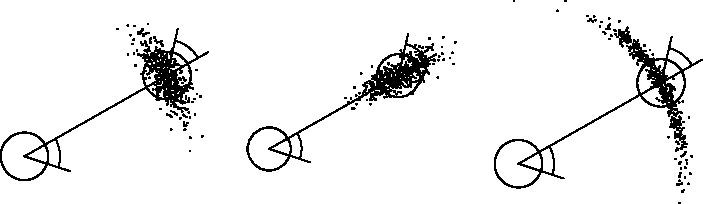
\includegraphics[width=0.6\columnwidth]{./images/samping_odometry_motion_model.pdf}
    	}\\
    	\subfloat[Muestras del motion model]
    	{
    		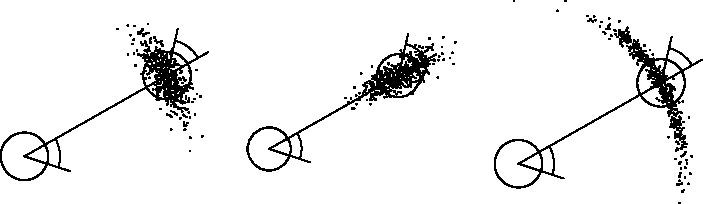
\includegraphics[width=0.6\columnwidth]{./images/samping_odometry_motion_model.pdf}
    	}
    \end{figure}


\end{frame}


\section{Medición}

\begin{frame}{Belief luego de sensar}
    \begin{block}{Ejemplo}
        \begin{itemize}
            \item Un mundo constituido por cinco celdas $x_{i}$ donde $i = 1, \dots ,5$
            \item Las celdas $x_{2}$ y $x_{3}$ son rojas, y el resto verdes.
            \item Inicialmente el robot desconoce su posición
            \item La probabilidad de que el robot sense correctamente  esta dada por la siguiente distribución de probabilidades:
            
            \begin{displaymath}
                P(sensa \ color | x_{i} = color) = 0.6
            \end{displaymath}
            \begin{displaymath}
                P(sensa \ \neg color | x_{i} = color) = 0.2
            \end{displaymath}
            
            Observar que no es una distribución de probabilidad correcta ya que la suma debe ser $1$.
            
        \end{itemize}
        
    \end{block}
    
    \begin{center}
        \includegraphics<1>[height=1.0cm]{./images/uniform_five_cells.png}
    \end{center}
    
\end{frame}

\begin{frame}{Belief luego de sensar}
    
    Si el robot \alert{sensa rojo}, ?`Cuál es su Posterior belief?
    
    \begin{center}
        \includegraphics<1>[height=3.5cm]{./images/inaccurate_sensing_quiz.png}
    \end{center}
\end{frame}

\begin{frame}{Belief luego de sensar}
    
    Si el robot \alert{sensa rojo}, ?`Cuál es su Posterior belief?
    
    \begin{center}
        \includegraphics<1>[height=3.5cm]{./images/inaccurate_sensing_solution.png}
    \end{center}
    \begin{footnotesize}
        \begin{displaymath}
            P(x_{i} = rojo | sensa \ rojo) = P(sensa \ rojo | x_{i} = rojo) P(x_{i}) = 0.2 \times 0.6 = 0.12
        \end{displaymath}
        \begin{displaymath}
            P(x_{i} = verde | sensa \ rojo) = P(sensa \ rojo | x_{i} = verde) P(x_{i}) = 0.2 \times 0.2 = 0.04
        \end{displaymath}
    \end{footnotesize}
    
\end{frame}

\begin{frame}{Belief luego de sensar}
    \begin{displaymath}
        P(x_{i} = rojo | sensa \ rojo) = 0.12
    \end{displaymath}
    \begin{displaymath}
        P(x_{i} = verde | sensa \ rojo) = 0.04
    \end{displaymath}
    
    Observar que estamos ante una distribución de probabilidades formalmente incorrecta dado que la suma: 
    \begin{displaymath}
        \sum_{i=1}^{5} P(x_{i}) = 0.04 + 0.12 + 0.12 + 0.04 + 0.04 = 0.36
    \end{displaymath}
    
    
    Si normalizamos la distribución, queda:
    
    \begin{displaymath}
        P(x_{i} = rojo| sensa \ rojo) = \dfrac{0.12}{0.36} = \dfrac{1}{3}
    \end{displaymath}
    \begin{displaymath}
        P(x_{i} = verde| sensa \ rojo) = \dfrac{0.04}{0.36} = \dfrac{1}{9}
    \end{displaymath}
    
    En general, $P(x_{i}|z)$ es la distribución Posterior belief del lugar $x_{i}$ dada la medición $z$.
\end{frame}


\begin{frame}{Regla de Bayes}
    
    Notar que cuando el robot sensa no hace otra cosa que aplicar la Regla Bayes:
    
    \begin{block}{Regla de Bayes}
        \begin{displaymath}
            P(x_{i} | z) = \dfrac{P(z | x_{i})P(x_{i})} {P(z)} 
        \end{displaymath}
        $P(x_{i} | z)$ : probabilidad a Posteriori (Posterior Belief) \\
        $P(z | x_{i})$ : probabilidad de Medición \\
        $P(x_{i})$ : probabilidad a Priori \\
        $P(z)$ : término de Normalización
    \end{block}
    
\end{frame}

\section{Motricidad}
\begin{frame}{Belief luego del movimiento}
    \begin{block}{Ejemplo (continuación)}
        \begin{itemize}
            \item Un mundo \alert{cíclico} constituido por cinco celdas $x_{i}$ donde $i = 1, \dots ,5$
            \item La distribución de probabilidad a priori esta determinada por:
            \begin{displaymath}
                P(x_{1}) = P(x_{4}) = P(x_{5}) = \dfrac{1}{9}
            \end{displaymath}
            \begin{displaymath}
                P(x_{2}) = P(x_{3}) = \dfrac{1}{3}	
            \end{displaymath}
        \end{itemize}
    \end{block}
    
\end{frame}

\begin{frame}{Belief luego del movimiento}
    Si el robot tiene una \alert{motricidad exacta} y desea moverse \alert{una} celda a la derecha, ?`Cuál es su Posterior belief?
    
    \begin{center}
        \includegraphics<1>[height=3.5cm]{./images/exact_motion_quiz.png}
    \end{center}
    
\end{frame}

\begin{frame}{Belief luego del movimiento}
    Si el robot tiene una \alert{motricidad exacta} y desea moverse \alert{una} celda a la derecha, ?`Cuál es su Posterior belief?
    
    \begin{center}
        \includegraphics<1>[height=3.5cm]{./images/exact_motion_solution.png}
    \end{center}
    
\end{frame}

\begin{frame}{Belief luego del movimiento}
    Suponiendo ahora que el robot desea moverse \alert{dos} celdas a la derecha y tiene una \alert{motricidad inexacta} con la siguiente distribución de probabilidad:
    \begin{columns}[t]
        \begin{column}{5cm}
            \begin{displaymath}
                P(x_{i+2}| x_{i}) = 0.8
            \end{displaymath}
            \begin{displaymath}
                P(x_{i+1}| x_{i}) = 0.1
            \end{displaymath}
            \begin{displaymath}
                P(x_{i+3}| x_{i}) = 0.1
            \end{displaymath}
        \end{column}
        \begin{column}{5cm}
            \begin{center}
                \includegraphics<1>[height=1.8cm]{./images/inexact_motion.png}
            \end{center}
        \end{column}
    \end{columns}
\end{frame}

\begin{frame}{Belief luego del movimiento}
    
    Si el robot conoce exactamente cuál es su posición inicial, ?`Cuál es su Posterior belief?
    
    \begin{columns}[t]
        \begin{column}{5cm}
            \begin{center}
                \includegraphics<1>[height=2.0cm]			{./images/inexact_motion_initial_pose_quiz.png}
            \end{center}
        \end{column}
        \begin{column}{5cm}
            \begin{center}
                \includegraphics<1>[height=1.8cm]{./images/inexact_motion.png}
            \end{center}
        \end{column}
    \end{columns}
\end{frame}

\begin{frame}{Belief luego del movimiento}
    
    Si el robot conoce exactamente cuál es su posición inicial, ?`Cuál es su Posterior belief?
    
    \begin{columns}[t]
        \begin{column}{5cm}
            \begin{center}
                \includegraphics<1>[height=2cm]			{./images/inexact_motion_initial_pose_solution.png}
            \end{center}
        \end{column}
        \begin{column}{5cm}
            \begin{center}
                \includegraphics<1>[height=1.8cm]{./images/inexact_motion.png}
            \end{center}
        \end{column}
    \end{columns}
\end{frame}

\begin{frame}{Belief luego del movimiento}
    Si el robot tiene como distribución inicial que se encuentra en las celdas $x_{2}$ y $x_{4}$ con igual probabilidad, formalmente,
    \begin{displaymath}
        P(x_{2}) = P(x_{4}) = 0.5
    \end{displaymath}
    ?`Cuál es su Posterior belief?
    
    \begin{columns}[t]
        \begin{column}{5cm}
            \begin{center}
                \includegraphics<1>[height=2cm]{./images/inexact_motion_quiz.png}
            \end{center}
        \end{column}
        \begin{column}{5cm}
            \begin{center}
                \includegraphics<1>[height=1.8cm]{./images/inexact_motion.png}
            \end{center}
        \end{column}
    \end{columns}
\end{frame}

\begin{frame}{Belief luego del movimiento}
    
    Si el robot tiene como distribución inicial que se encuentra en las celdas $x_{2}$ y $x_{4}$ con igual probabilidad, formalmente,
    \begin{displaymath}
        P(x_{2}) = P(x_{4}) = 0.5
    \end{displaymath}
    ?`Cuál es su Posterior belief?
    
    \begin{columns}[t]
        \begin{column}{5cm}
            \begin{center}
                \includegraphics<1>[height=2cm]{./images/inexact_motion_solution.png}
            \end{center}
        \end{column}
        \begin{column}{5cm}
            \begin{center}
                \includegraphics<1>[height=1.8cm]{./images/inexact_motion.png}
            \end{center}
        \end{column}
    \end{columns}
    \begin{small}
        $P(x_{1}) = P(x_{4}) P(x_{1}|x_{4}) = 0.5 \times 0.8 = 0.4$ \\
        $P(x_{2}) = P(x_{4}) P(x_{2}|x_{4}) = 0.5 \times 0.1 = 0.05$ \\
        $P(x_{3}) = P(x_{2}) P(x_{3}|x_{2}) = 0.5 \times 0.1 = 0.05$ \\	
        $P(x_{4}) = P(x_{2}) P(x_{4}|x_{2}) = 0.5 \times 0.8 = 0.4$ \\	
        $P(x_{5}) = P(x_{2}) {\color{red} P(x_{5}|x_{2})} + P(x_{4}) {\color{green} P(x_{5}|x_{4})} = 0.5 \times {\color{red} 0.1} + 0.5 \times {\color{green} 0.1} = 0.1$	
    \end{small}
\end{frame}

\section{Sensar y Mover}
\begin{frame}{Ciclo de sensar y mover}
    Localización no es más que la iteración de sensar y mover.
    \begin{center}
        \includegraphics<1>[height=2.5cm]{./images/sens_and_move.pdf}
    \end{center}
    
    \begin{block}{Entropía}
        Medida de información que tiene la distribución
        \begin{displaymath}
            - \sum P(x_{i}) \log P(x_{i})
        \end{displaymath}
        
        En otras palabras, la entropía expresa la información que un robot recibe luego de ejecutar una acción específica.
    \end{block}
    
\end{frame}


\begin{frame}{Definición formal de localización}
    
    \begin{block}{Medición}
        \begin{displaymath}
            \Bar{P}(x_{i}|z) \leftarrow P(z|x_{i}) P(x_{i})
        \end{displaymath}
        \begin{displaymath}
            \alpha \leftarrow \sum \Bar{P}(x_{i}|z)
        \end{displaymath}
        \begin{displaymath}
            P(x_{i}|z) \leftarrow \frac{1}{\alpha} \Bar{P}(x_{i}|z)
        \end{displaymath}
        
    \end{block}
    
\end{frame}

\begin{frame}{Definición formal de localización}
    
    Sea $P(x_{i}^{t})$ la probabilidad de estar en el punto $x_{i}$ luego del movimiento del robot
    
    \begin{block}{Motricidad}
        
        \begin{displaymath}
            P(x_{i}^{t}) = \sum_{j} P(x_{j}^{t-1}) P(x_{i}|x_{j})
        \end{displaymath}
        
    \end{block}
    
    La probabilidad de estar en $x_{i}$ se calcula a través de todos los lugares de los que podríamos haber venido
    
    Observar que la expresión anterior no es otra cosa que el Teorema de Probabilidad total.
    
    \begin{block}{Teorema de Probabilidad Total}
        
        \begin{displaymath}
            P(A) = \sum_{B}^{}P(A|B) P(B)
        \end{displaymath}
        
    \end{block}
    
\end{frame}


\begin{frame}
	\frametitle{Bayes Filter}
	
	\note{Información obtenida de Cyrill Stachniss Bayes: https://youtu.be/0lKHFJpaZvE}
	
	
\end{frame}

\begin{frame}
	\frametitle{Extended Kalman Filter}
	
	\note{Información obtenida de:
		Cyrill Stachniss KF y EKF: https://youtu.be/E-6paM_Iwfc
		Chebrolu EKF Localization: https://youtu.be/PiCC-SxWlH8}
    
    https://automaticaddison.com/extended-kalman-filter-ekf-with-python-code-example/
    https://github.com/shangzhouye/EKF-SLAM-on-Turtlebot3
    
    https://github.com/ser94mor/sensor-fusion
    
    https://github.com/AtsushiSakai/PythonRobotics
    
    Puede ser que el tp sea en python no mas y el tp final hacerlo en ROS2.
    
    https://github.com/debbynirwan/mcl
    
    
\end{frame}


	
	\section{Filtro de Kalman Extendido (EKF)}
	\begin{frame}
	\frametitle{Kalman Filter}
	\note{información extraida de https://youtu.be/PiCC-SxWlH8}
	
	\begin{itemize}
		\item Es un Filtro de Bayes
		\item Todo es Gaussiano
		\begin{equation*}
			p(x)=\det(2\pi\covariance)^{\frac{1}{2}} \exp\left(-\dfrac{1}{2} (x - \mu )^{\top} \inverse{\covariance} (x - \mu )  \right)
		\end{equation*}
		
		\item Soluciones optimas para modelos lineales y distribuciones Gaussianas.
	\end{itemize}

	\begin{figure}[!h]
		\centering
		\subfloat[]
		{
			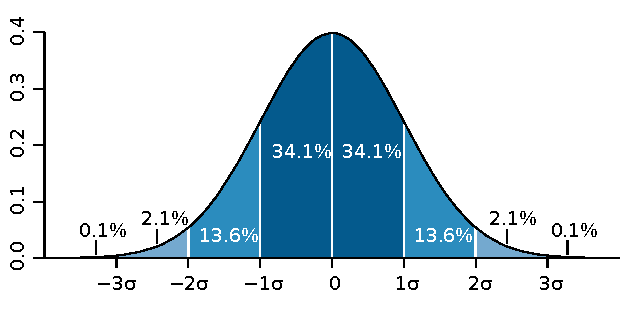
\includegraphics[width=0.3\columnwidth]{./images/standard_deviation_diagram.pdf}
		}
		\subfloat[AGREGAR ELIPSE ELIPSOIDE ]
		{
			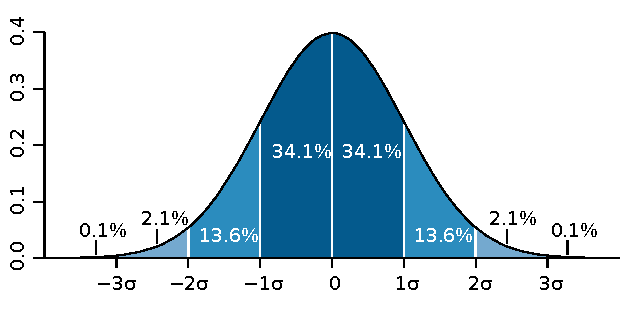
\includegraphics[width=0.3\columnwidth]{./images/standard_deviation_diagram.pdf}
		}
	\end{figure}
\end{frame}


\begin{frame}
	\frametitle{Kalman Filter Asunciones}
	\note{información extraida de https://youtu.be/PiCC-SxWlH8}
	
	\begin{itemize}
		\item Ruido y distribuciones Gaussianas
		\item Modelos de movimiento y observación lineales
	\end{itemize}

	\begin{align*}
		\state_{t} &= A_{t} \state_{t-1} + B_{t}\controlCommand_{t} + \motionModelNoise_{t}\\
		\observation_{t} &= C_{t} \state_{t} + \measurementModelNoise_{t}
	\end{align*}
	\note{Kalman Filter requiere que los ruidos sean gaussianos y que el estado resulte de una combinación lineal.}

	\centering
	\alert{¿qué pasa si este estas asunciones no pasan?}
	\note{Differencial drive y Ackerman motion models NO son modelos lineales}
	\note{Los observation models de un láser  o de una cámara tampoco son lineales.}
\end{frame}

\begin{frame}
	\frametitle{Sistemas dinámicos no Non-lineales}
	\note{información extraida de https://youtu.be/PiCC-SxWlH8}
	\begin{itemize}
		\item Los problemas reales en general emplean funciones no-lineales
	\end{itemize}
	
	\begin{align*}
		\state_{t} &= A_{t} \state_{t-1} + B_{t}\controlCommand_{t} + \motionModelNoise_{t}\\
		\observation_{t} &= C_{t} \state_{t} + \measurementModelNoise_{t}
	\end{align*}

\TODO{tachar las formulas lineales}

	\begin{align*}
		\state_{t} &= \motionModelFunction{\controlCommand_{t}, \state_{t-1}} + \motionModelNoise_{t}\\
		\observation_{t} &= \observationModelFunction{\state_{t}} + \measurementModelNoise_{t}
	\end{align*}

\end{frame}

\begin{frame}
	\frametitle{Modelo de movimiento linearizado}
	\note{información extraida de https://youtu.be/PiCC-SxWlH8}
	
	\begin{itemize}
		\item Linearizar el modelo esta dado por:
	\begin{align*}
		p(\state_{t} | \controlCommand_{t}, \state_{t-1}) &\approx \det(2 \pi \motionParametersCovariance_{t})^{\frac{1}{2}}\\
		&\exp (-\dfrac{1}{2} (\state_{t} - \motionModelFunction{\controlCommand_{t}-\mu_{t-1}} - \motionModelJacobian_{t}(\state_{t-1}-\mu_{t-1}))^{\top}\\
		&\inverse{\motionParametersCovariance_{t}} (\state_{t} - \underbrace{\motionModelFunction{\controlCommand_{t},\mu_{t-1}} - \motionModelJacobian_{t} (\state_{t-1}-\mu_{t-1})}_{\text{modelo linearizado}}))
	\end{align*}
	
	\item $\motionParametersCovariance_{t}$ describe el ruido del movimiento
	\end{itemize}	
\end{frame}

\begin{frame}
	\frametitle{Modelo de observación linearizado}
	\note{información extraida de https://youtu.be/PiCC-SxWlH8}
	
	\begin{itemize}
		\item Linearizar el modelo esta dado por:
		\begin{align*}
			p(\observation_{t} | \state_{t}) &\approx \det(2 \pi \observationModelCovariance_{t})^{\frac{1}{2}}\\
			&\exp (-\dfrac{1}{2} (\observation_{t} - \observationModelFunction{\overline{\mu_{t}}} - \observationModelJacobian_{t}(\state_{t} - \overline{\mu_{t}}))^{\top}\\
			&\inverse{\observationModelCovariance_{t}} (\observation_{t} - \underbrace{\observationModelFunction{\overline{\mu_{t}}} - \observationModelJacobian_{t} (\state_{t}-\overline{\mu_{t}})}_{\text{modelo linearizado}}))
		\end{align*}
		
		\item $\observationModelCovariance_{t}$ describe el ruido de la medición
	\end{itemize}	
	
	
\end{frame}

\begin{frame}
	\frametitle{Algoritmo de Filtro de Kalman Extendido}
	\note{información extraída de https://youtu.be/PiCC-SxWlH8}
	
    \begin{algorithmic}[1]
    \Procedure{ExtendedKalmanFilter}{$\mu_{t-1}, \covariance_{t-1}, \controlCommand_{t}, \observation_{t}$}
        \State $\overline{\mu}_{t} = \motionModelFunction{\controlCommand_{t}, \mu_{t-1}}$
        \State $\overline{\covariance}_{t} = \motionModelJacobian_{t} \covariance_{t-1} \motionModelJacobian_{t}^{\top}+\motionParametersCovariance_{t}$
        \Statex
        \State $\kalmanGain_{t} = \overline{\covariance}_{t} \observationModelJacobian_{t}^{\top} (\observationModelJacobian_{t} \overline{\covariance}_{t}  \observationModelJacobian_{t} + \observationModelCovariance_{t})^{-1} $
        \State $\mu_{t} = \overline{\mu}_{t} + \kalmanGain_{t} (\observation_{t} - \observationModelFunction{\overline{\mu}_{t}})$
        \State $\covariance_{t} =  (I - \kalmanGain_{t} \observationModelJacobian_{t}) \overline{\covariance}_{t}$
        \State \Return $\mu_{t}, \covariance_{t}$
    \EndProcedure
    \end{algorithmic}
\end{frame}

\section{EKF Localización for feature-based map}

\begin{frame}
	\frametitle{Odometry as controls}
	\note{información extraida de https://youtu.be/PiCC-SxWlH8}
	
   	\begin{figure}[!h]
        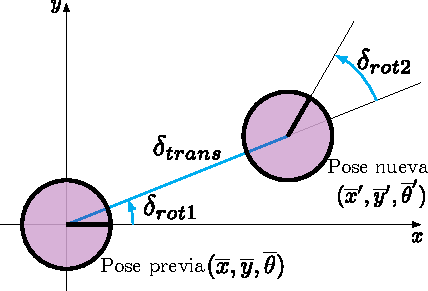
\includegraphics[width=0.6\columnwidth]{./images/odometry_as_controls.pdf}
    \end{figure}

    \begin{equation*}
        \controlCommand = (\delta_{rot1}, \delta_{trans}, \delta_{rot2})
    \end{equation*}
	
\end{frame}

\begin{frame}
	\frametitle{Motion model}
	\note{información extraida de https://youtu.be/PiCC-SxWlH8}
	
	\begin{itemize}
		\item Odometría de modelo de movimiento
		\begin{equation*}
			\begin{bmatrix}
				x^{\prime} \\
				y^{\prime} \\
				\theta^{\prime}
			\end{bmatrix} =
			\underbrace{
				\begin{bmatrix}
				x \\
				y \\
				\theta
			\end{bmatrix} +
			\begin{bmatrix}
				\delta_{trans}\cos(\theta+\delta_{rot_{1}}) \\
				\delta_{trans}\cos(\theta+\delta_{rot_{1}}) \\
				\delta_{rot_{1}} + \delta_{rot_{2}}
			\end{bmatrix}
			}_{\motionModelFunction{\controlCommand_{t}, \state_{t-1}}} + \normalDistribution{0}{\motionParametersCovariance_{t}}
		\end{equation*}
		\item Linearización
		\begin{equation*}
			\motionModelFunction{\controlCommand_{t}, \state_{t-1}} \approx 			\motionModelFunction{\controlCommand_{t}, \mu_{t-1}} + \covariance_{t}(\state_{t-1}-\mu_{t-1})
		\end{equation*}
	\end{itemize}
	
\end{frame}

\begin{frame}
	\frametitle{Jacobianos del modelo de movimiento}
	\note{información extraida de https://youtu.be/PiCC-SxWlH8}
	Calculamos el Jacobiano con respecto al estado
	\begin{equation*}
		\motionModelJacobian_{t} = \dfrac{\delta\motionModelFunction{\controlCommand_{t},\mu_{t-1}}}{\delta \state_{t-1}} =
		\begin{bmatrix}
			\dfrac{\delta x^{\prime}}{\delta \mu_{t-1,x}} & \dfrac{\delta x^{\prime}}{\delta \mu_{t-1,y}} & \dfrac{\delta x^{\prime}}{\delta \mu_{t-1,\theta}}\\
			\dfrac{\delta y^{\prime}}{\delta \mu_{t-1,x}} & \dfrac{\delta y^{\prime}}{\delta \mu_{t-1,y}} & \dfrac{\delta y^{\prime}}{\delta \mu_{t-1,\theta}}\\
			\dfrac{\delta \theta^{\prime}}{\delta \mu_{t-1,x}} & \dfrac{\delta \theta^{\prime}}{\delta \mu_{t-1,y}} & \dfrac{\delta \theta^{\prime}}{\delta \mu_{t-1,\theta}}\\
		\end{bmatrix}
	\end{equation*}

	\begin{equation*}
	\motionModelJacobian_{t} = 
	\begin{bmatrix}
		1 & 0 & -\delta_{trans} \sin(\theta + \delta_{rot_{1}})\\
		0 & 1 & \delta_{trans} \cos(\theta + \delta_{rot_{1}})\\
		0 & 0 & 1\\
	\end{bmatrix}
	\end{equation*}
\end{frame}

\begin{frame}
	\frametitle{Jacobianos del modelo de movimiento}
	\note{información extraida de https://youtu.be/PiCC-SxWlH8}
	Calculamos el Jacobiano con respecto al comando de control
	\begin{equation*}
		\motionModelJacobianControl{t} = \dfrac{\delta\motionModelFunction{\controlCommand_{t},\mu_{t-1}}}{\delta \controlCommand_{t}} =
		\begin{bmatrix}
			\dfrac{\delta x^{\prime}}{\delta \controlCommand_{t,\delta_{rot_{1}}}} & \dfrac{\delta x^{\prime}}{\delta \controlCommand_{t,\delta_{trans}}} & \dfrac{\delta x^{\prime}}{\delta \controlCommand_{t,\delta_{rot_{2}}}}\\
			\dfrac{\delta y^{\prime}}{\delta \controlCommand_{t,\delta_{rot_{1}}}} & \dfrac{\delta y^{\prime}}{\delta \controlCommand_{t,\delta_{trans}}} & \dfrac{\delta y^{\prime}}{\delta \controlCommand_{t,\delta_{rot_{2}}}}\\
			\dfrac{\delta \theta^{\prime}}{\delta \controlCommand_{t,\delta_{rot_{1}}}} & \dfrac{\delta \theta^{\prime}}{\delta \controlCommand_{t,\delta_{trans}}} & \dfrac{\delta \theta^{\prime}}{\delta \controlCommand_{t,\delta_{rot_{2}}}}
		\end{bmatrix}
	\end{equation*}
	
	\begin{equation*}
		\motionModelJacobianControl_{t} = 
		\begin{bmatrix}
			-\delta_{trans} \sin(\theta + \delta_{rot_{1}}) & \cos(\theta + \delta_{rot_{1}}) & 0\\
			\delta_{trans} \cos(\theta + \delta_{rot_{1}}) & \sin(\theta + \delta_{rot_{1}}) & 0\\
			0 & 0 & 1\\
		\end{bmatrix}
	\end{equation*}
\end{frame}

\begin{frame}
	\frametitle{Modelo de observación}
	\note{información extraida de https://youtu.be/PiCC-SxWlH8}
	\begin{itemize}
	\item Modelo de distancia y orientación (range-bearing model)
	\begin{equation*}
		\observation_{t}^{i} =
		\begin{bmatrix}
			r_{t}^{i}\\
			\phi_{t}^{i} 
		\end{bmatrix} =
		\begin{bmatrix}
			\sqrt{(m_{j,x}-x)^{2} + (m_{j,y}-y)^{2}}\\
			\atantwo(m_{j,y}-y, m_{j,x}-x) -\theta
		\end{bmatrix}
		+ \normalDistribution{0}{\observationModelCovariance_{t}}		
	\end{equation*}
	
	\item Linearización
	\begin{equation*}
	\observationModelFunction{\state_{t}, m} \approx 			\observationModelFunction{\overline{\mu}_{t}} + \observationModelJacobian_{t}^{i}(\state_{t}-\overline{\mu}_{t})
	\end{equation*}
	\end{itemize}
	
\end{frame}

\begin{frame}
	\frametitle{Jacobianos del modelo de observación}
	\note{información extraida de https://youtu.be/PiCC-SxWlH8}
	Calculamos el Jacobiano con respecto al estado
	\begin{equation*}
		\observationModelJacobian_{t} = \dfrac{\delta\observationModelFunction{\overline{\mu}_{t},m}}{\delta \state_{t-1}} =
		\begin{bmatrix}
			\dfrac{\delta r_{t}^{i}}{\delta \overline{\mu}_{t,x}} & \dfrac{\delta r_{t}^{i}}{\delta \overline{\mu}_{t,y}} & \dfrac{\delta r_{t}^{i}}{\delta \overline{\mu}_{t,\theta}}\\
			\dfrac{\delta \phi_{t}^{i}}{\delta \overline{\mu}_{t,x}} & \dfrac{\delta \phi_{t}^{i}}{\delta \overline{\mu}_{t,y}} & \dfrac{\delta \phi_{t}^{i}}{\delta \overline{\mu}_{t,\theta}}
		\end{bmatrix}
	\end{equation*}
	
	\begin{equation*}
		\observationModelJacobian_{t}^{i} = 
		\begin{bmatrix}
			-\dfrac{m_{j,x} - \overline{\mu}_{t,x}}{\sqrt{q}} & -\dfrac{m_{j,y} - \overline{\mu}_{t,y}}{\sqrt{q}}  & 0\\
			-\dfrac{m_{j,y} - \overline{\mu}_{t,y}}{q}  & -\dfrac{m_{j,x} - \overline{\mu}_{t,x}}{q}  & -1
		\end{bmatrix}
	\end{equation*}
	donde
	\begin{equation*}
		q = (m_{j,x}-\overline{\mu}_{t,x})^{2} + (m_{j,y}-\overline{\mu}_{t,y})^{2}
	\end{equation*}
\end{frame}

\begin{frame}
	\frametitle{Algoritmo de Filtro de Kalman Extendido}
	\note{información extraida de https://youtu.be/PiCC-SxWlH8}
	
 	\begin{algorithmic}[1]
		\State ExtendedKalmanFilter({$\mu_{t-1}, \covariance_{t-1}, \controlCommand_{t}, \observation_{t}$, $c_{t}$, $m$})
		\State $\theta = \mu_{t-1,\theta}$
		
		\State $
			\motionModelJacobian_{t} = 
			\begin{bmatrix}
				1 & 0 & -\delta_{trans} \sin(\theta + \delta_{rot_{1}})\\
				0 & 1 & \delta_{trans} \cos(\theta + \delta_{rot_{1}})\\
				0 & 0 & 1\\
			\end{bmatrix}
			   $
		\State $
			\motionModelJacobianControl_{t} = 
			\begin{bmatrix}
				-\delta_{trans} \sin(\theta + \delta_{rot_{1}}) & \cos(\theta + \delta_{rot_{1}}) & 0\\
				\delta_{trans} \cos(\theta + \delta_{rot_{1}}) & \sin(\theta + \delta_{rot_{1}}) & 0\\
				0 & 0 & 1\\
			\end{bmatrix}
         	   $
		\State $
			\motionModelCovariance_{t} = 
			\begin{bmatrix}
				\alpha_{1}\delta^{2}_{rot_{1}} + \alpha_{2}\delta^{2}_{trans} & 0 & 0\\
				0 & \alpha_{3} \delta^{2}_{trans} + \alpha_{4} \left( \delta^{2}_{rot_{1}} + \delta^{2}_{rot_{2}} \right) & 0\\
				0 & 0 & \alpha_{1}\delta^{2}_{rot_{1}} + \alpha_{2}\delta^{2}_{trans}\\
			\end{bmatrix}
			  $
		\State $\overline{\mu}_{t} = \mu_{t-1} + 
			\begin{bmatrix}
			\delta_{trans}\cos(\theta+\delta_{rot_{1}}) \\
			\delta_{trans}\cos(\theta+\delta_{rot_{1}}) \\
			\delta_{rot_{1}} + \delta_{rot_{2}}
		\end{bmatrix}$
		\State $\overline{\covariance}_{t} = \motionModelJacobian_{t} \covariance_{t-1} \motionModelJacobian_{t}^{\top}+\motionModelJacobianControl_{t} \motionModelCovariance_{t} \motionModelJacobianControl_{t}^{\top}$
	\end{algorithmic}
	
\end{frame}

\begin{frame}
	\frametitle{Prediction step}
	\note{información extraida de https://youtu.be/PiCC-SxWlH8}
	
	\begin{figure}[!h]
		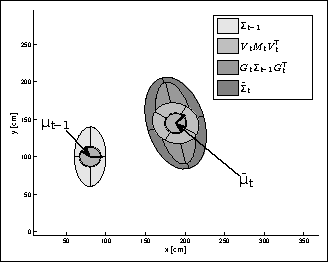
\includegraphics[width=0.5\columnwidth]{./images/prediction_step.pdf}
	\end{figure}
	
\end{frame}

\begin{frame}
	\frametitle{Algoritmo de Filtro de Kalman Extendido}
	\note{información extraida de https://youtu.be/PiCC-SxWlH8}
	\footnotesize
 	\begin{algorithmic}[1]
		\State
		$ \observationModelCovariance_{t} =
			\begin{bmatrix}
				\sigma_{r}^{2} & 0\\
				0 & \sigma_{\phi}^{2}
			\end{bmatrix}
		$
		\For todos los features observados $z_{t}^{i} = (r_{t}^{i}, \phi_{t}^{i})^{\top}$
		
		\State $ j = c_{t}^{i}$
		\State $ q = (m_{j,x}-\overline{\mu}_{t,x})^{2} + (m_{j,y}-\overline{\mu}_{t,y})^{2} $
		\State
		$ \hat{\observation}_{t}^{i} =
			\begin{bmatrix}
				\sqrt{q}\\
				\atantwo(m_{j,y}-\overline{\mu}_{t,y}, m_{j,x}-\overline{\mu}_{t,x}) - \overline{\mu}_{t,\theta}
			\end{bmatrix}
		$
		\State
		$ \observationModelJacobian_{t}^{i} = 
			\begin{bmatrix}
				-\dfrac{m_{j,x} - \overline{\mu}_{t,x}}{\sqrt{q}} & -\dfrac{m_{j,y} - \overline{\mu}_{t,y}}{\sqrt{q}}  & 0\\
				-\dfrac{m_{j,y} - \overline{\mu}_{t,y}}{q}  & -\dfrac{m_{j,x} - \overline{\mu}_{t,x}}{q}  & -1
			\end{bmatrix}
		$
		
		\State $S_{t}^{i} = \observationModelJacobian_{t}^{i} \overline{\covariance}_{t} \observationModelJacobian_{t}^{i^{\top}} + \observationModelCovariance_{t} $

		\State $\kalmanGain_{t}^{i} = \overline{\covariance}_{t} {\observationModelJacobian_{t}^{i}} \overline{\covariance}_{t} \observationModelJacobian_{t}^{i^{\top}} S_{t}^{i^{-1}} $
		\State $\overline{\mu}_{t} = \overline{\mu}_{t} + \kalmanGain_{t}^{i}(\observation_{t} - \hat{\observation}_{t}^{i})$
		\State $\overline{\covariance}_{t} = (I - \kalmanGain_{t}^{i}\observationModelJacobian_{t}^{i})\overline{\covariance}_{t}$
		
		\EndFor
		\State $\mu_{t} = \overline{\mu}_{t}$
		\State $\covariance_{t} = \overline{\covariance}_{t}$
		
		\State \Return $\mu_{t}, \covariance_{t}$
	\end{algorithmic}
	
	
\end{frame}

\begin{frame}
	\frametitle{Medición esperada}
	\note{información extraida de https://youtu.be/PiCC-SxWlH8}
	
	\begin{figure}[!h]
		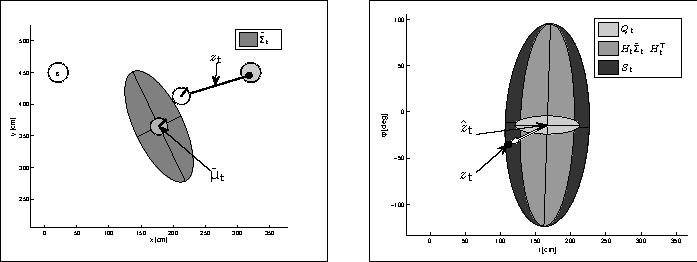
\includegraphics[width=\columnwidth]{./images/measurement_prediction.pdf}
	\end{figure}
	
\end{frame}

\begin{frame}
	\frametitle{Correction step}
	\note{información extraida de https://youtu.be/PiCC-SxWlH8}
	
	\begin{figure}[!h]
			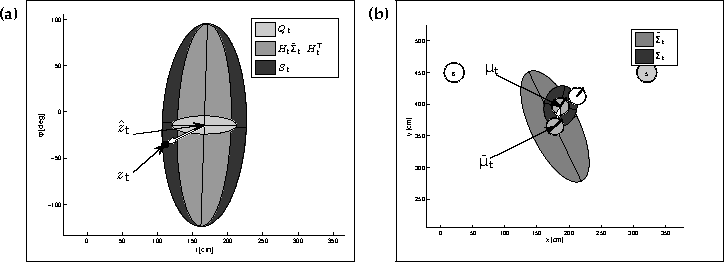
\includegraphics[width=\columnwidth]{./images/correction_step.pdf}
	\end{figure}
	
\end{frame}

\begin{frame}
	\frametitle{Ejemplo: EKF Localization 2D}
	\note{información extraida de libro Probabilistic Robotics}
	
	\begin{figure}[!h]
		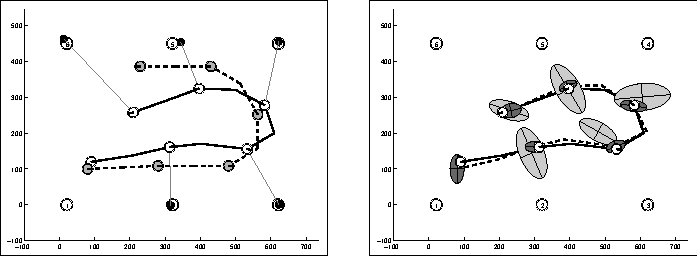
\includegraphics[width=\columnwidth]{./images/ekf_localization_example.pdf}
	\end{figure}
	
\end{frame}

\begin{frame}
	\frametitle{Resumen de EKF}
	\note{información extraida de https://youtu.be/PiCC-SxWlH8}
	
	\begin{itemize}
		\item Es una extensión del Filtro de Kalman
		\item Una forma de trabajar con no-lineridades
		\item Realiza linearizaciones locales
		\item Funciona bien en la práctica para casos moderadamente no lineales
		\item Grandes incertidumbres conllevan un incremento del error
	\end{itemize}
	
\end{frame}



   	\section{Filtro de Partículas}
    \begin{frame}
    \frametitle{Filtro de Partículas (Particle Filter)}
    \note{Información extraída de Vídeo de Cyrill Stachniss https://youtu.be/MsYlueVDLI0}
    \footnotesize
    \begin{itemize}
        \item Con EKF estamos restringidos a distribuciones Gaussianas.
        \item Cuando usamos EKF obtenemos una Distibuión Gaussiana que describe dónde se encuentra el robot.
        \item En Particle Filter utilizamos partículas o hipótesis que describen dónde podría estar el robot.
        \item En vez de tener una forma paramétrica como es EKF, que describimos la distribución de probabilidad con los parámetros media $\mu$ y covarianza $\covariance$. Partible Filter utiliza muestras no-paramétricas como hipótesis sobre dónde el robot podría estar.
    \end{itemize}
    
    
   	\begin{center}
        \movie[loop]{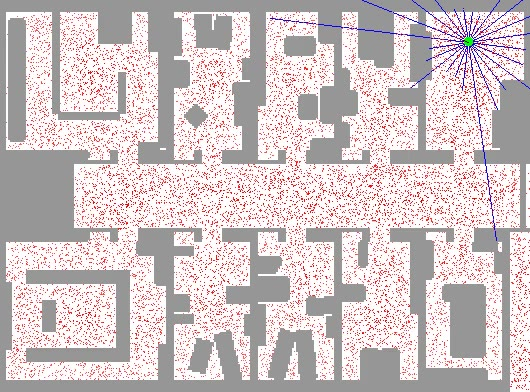
\includegraphics[width=0.4\columnwidth]{images/particle_filter/particle_filter_video.jpg}}{videos/particle_filter.mp4}
    \end{center}
    
    \note{Vídeo extraído de https://rse-lab.cs.washington.edu/projects/mcl/animations/global-floor.gif}
    
\end{frame}

\begin{frame}
    \frametitle{Aproximación de una Función}
    \note{Información extraída de Vídeo de Cyrill Stachniss https://youtu.be/MsYlueVDLI0}
    \footnotesize
    
    \begin{itemize}
        \item Objetivo: Poder estimar cualquier \textbf{distribución de probabilidad arbitraria}.
    \end{itemize}
    
    \begin{center}
    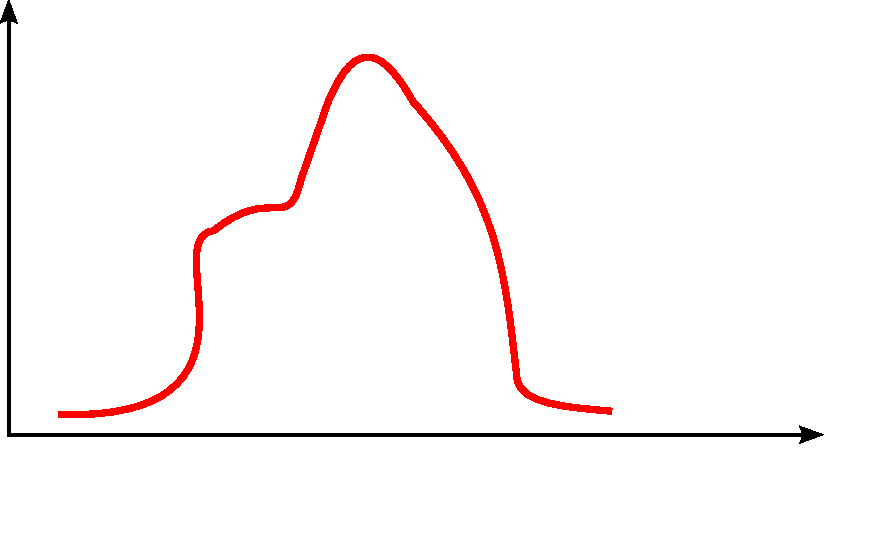
\includegraphics[width=0.5\columnwidth]{./images/particle_filter/arbitrary_distribution.pdf}
    \end{center}
    
\end{frame}

\begin{frame}
    \frametitle{Utilizando Muestras (Partículas)}
    \note{Información extraída de Vídeo de Cyrill Stachniss https://youtu.be/MsYlueVDLI0}
    \footnotesize
    \begin{itemize}
        \item \textbf{Múltiples muestras} para representar una distribución de probabilidad arbitraría
        \item Las muestras son están más agrupadas en algunas áreas en otras menos. La cantidad de partículas por unidad de área describe que tan probable es que el robot se encuentre en esa área.
        \item Cada muestra está acumulando un poco de ``masa de probabilidad''.
        \item Las muestra puede ser vista como una aproximación a la función de densidad de probabilidad (pdf).
        \item Para obtener la pdf, hay que integrar sobre una cierta área de manera de obtener la probabilidad matemática de que el robot se encuentre en dicha área.
    \end{itemize}
    
    \begin{center}
    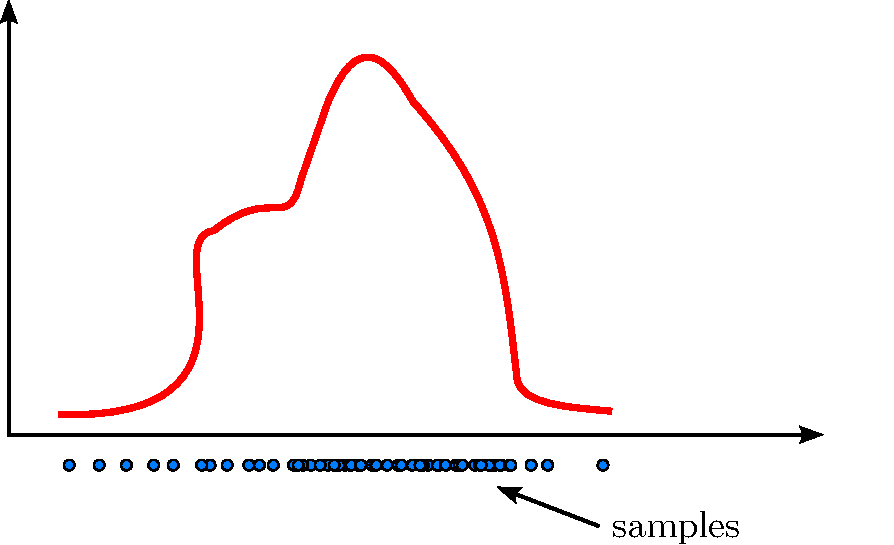
\includegraphics[width=0.5\columnwidth]{./images/particle_filter/arbitrary_distribution_samples.pdf}
    \end{center}
    
\end{frame}

\begin{frame}
    \frametitle{Utilizando Muestras con Peso}
    \note{Información extraída de Vídeo de Cyrill Stachniss https://youtu.be/MsYlueVDLI0}
    \footnotesize
    \begin{itemize}
        \item \textbf{Múltiples muestras con peso} para representar una distribución de probabilidad arbitraría
        \item Es posible reducir el número de muestras que necesitamos, si le agregamos pesos a cada muestra
        \item Mientras más peso tiene una muestra, más masa de probabilidad hay en esa región
        \item Los pesos de todas las partículas juntas deben sumar 1
        \item Al inicio, podríamos agregarle a cada muestra un peso uniforme. Por ejemplo, si tenemos $n$ muestras, entonces cada muestra tiene peso $\frac{1}{n}$
    \end{itemize}
    
    \begin{center}
        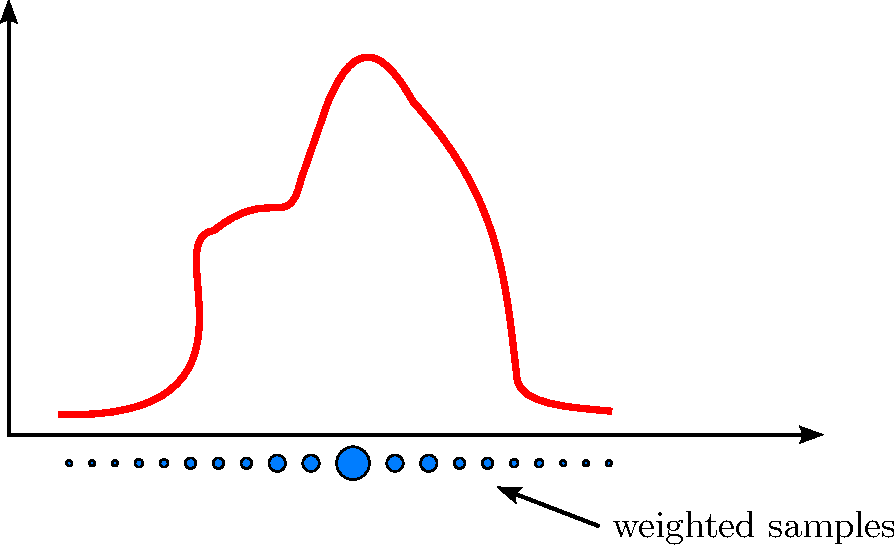
\includegraphics[width=0.5\columnwidth]{./images/particle_filter/arbitrary_distribution_weighted_samples.pdf}
    \end{center}
    
\end{frame}

\begin{frame}
    \frametitle{Filtro de Partículas (Particle Filter)}
    \note{Información extraída de Vídeo de Cyrill Stachniss https://youtu.be/MsYlueVDLI0}
    
    \footnotesize
    \begin{itemize}
        \item Notar que es una aproximación de la pdf
        \item Es importante tener un número de muestras suficientes para poder representar la fdp adecuadamente.
    \end{itemize}
    
    
\end{frame}

\begin{frame}
    \frametitle{Conjunto de Partículas}
    
    \begin{itemize}
        \item Conjunto de partículas con peso
            
        \begin{center}
            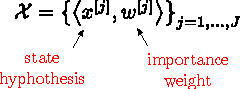
\includegraphics[width=0.5\columnwidth]{./images/particle_filter/weighted_samples.pdf}
        \end{center}

        \item Las partículas representan la posterior belief dada por
        \begin{equation*}
            p(x) = \sum_{j=1}^{J} w^{[j]} \delta_{x^{[j]}}(x)    
        \end{equation*}
        donde $\delta_{x^{[j]}}(x)$ es la función de Dirac centrada en la ubicación de la partícula $x^{[j]}$.

        \begin{equation*}
            \delta(y) = 
            \begin{cases} 
            \infty, & y = x^{[j]} \\ 
            0, & y \neq x^{[j]} 
            \end{cases};    
        \end{equation*}

        \note{La función tiende a infinito cuando $x=j$ y, para cualquier otro valor de $x$, es igual a 0.}

    \end{itemize}
   
\end{frame}


\begin{frame}
    \frametitle{Partículas para Aproximar}
    
    \begin{itemize}
        \item Partículas para aproximar una función
        
        \begin{center}
            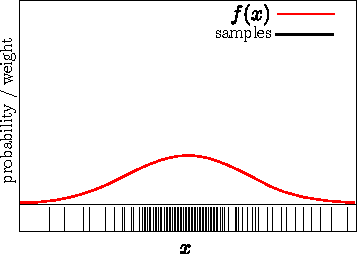
\includegraphics[width=0.45\columnwidth]{./images/particle_filter/gaussian_approximation_by_sampling.pdf}
            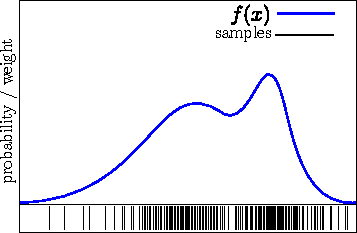
\includegraphics[width=0.45\columnwidth]{./images/particle_filter/particles_for_approximation.pdf}
        \end{center}

        \item Más partículas caen en una región, más alta es la probabilidad de la región
    \end{itemize}
    
    \begin{center}
        \alert{¿Cómo obtener dichas muestras?}
    \end{center}

\end{frame}

\begin{frame}
    \frametitle{Una Forma Cerrada de Muestreo es solo posible para Pocas Distribuciones }
    \begin{itemize}
        \item Ejemplo: Distribución Gaussiana
        
        \begin{center}
            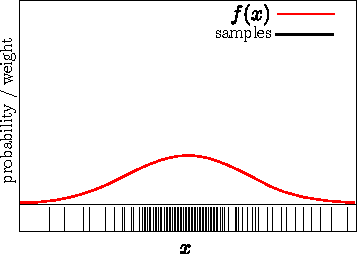
\includegraphics[width=0.5\columnwidth]{./images/particle_filter/gaussian_approximation_by_sampling.pdf}
        \end{center}
        
        \begin{equation*}
            x \leftarrow \frac{1}{2} \sum_{i=1}^{12} \text{rand}(-\sigma, \sigma)
        \end{equation*}
    \end{itemize}

    ¿Cómo samplear utilizando otra distribución?

    \note{Técnica de rejection sampling. No sé utiliza en particle filter porque es una técnica muy ineficiente.}

    \note{Técnica Importance Sampling Principle}

\end{frame}
    


\begin{frame}
    \frametitle{Principio de muestreo de importancia}
    \begin{itemize}
        \item Podemos usar una distribución diferente $\pi$ para generar muestras de $f$
        \item Considere las ``diferencias entre $\pi$ y $f$'' usando un peso $w = f(x) / \pi(x)$
        \item Target $f$
        \item Proposal $\pi$
        \item Precondición:
        $f(x) > 0 \implies \pi(x) > 0$
        \begin{center}
        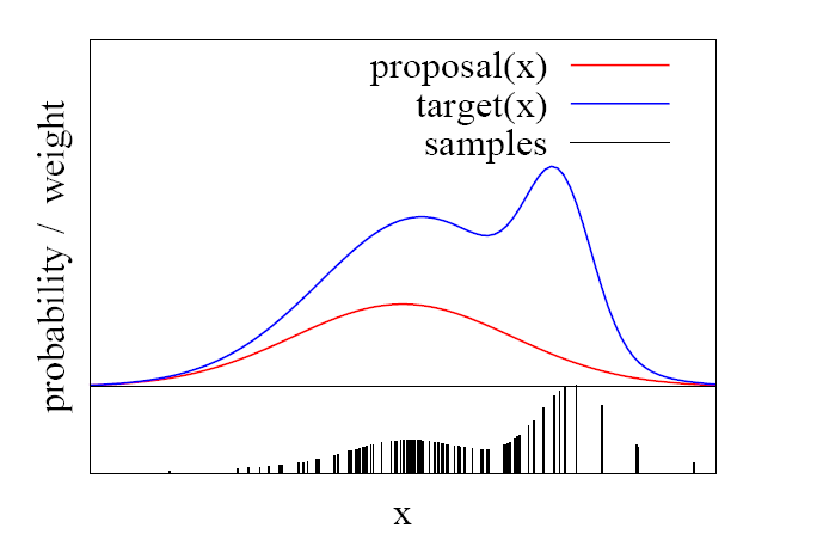
\includegraphics[width=0.45\textwidth]{./images/particle_filter/importance_sampling_principle.pdf}
        \end{center}
    \end{itemize}
\end{frame}
    
\begin{frame}
    \frametitle{Filtro de Partículas}
    \begin{itemize}
        \item Filtro Bayesiano recursivo
        \item Enfoque no paramétrico
        \item Modela la distribución mediante muestras
        \item \textbf{Predicción}: extraer de la distribución propuesta
        \item \textbf{Corrección}: ponderación por la relación entre la distribución objetivo y la propuesta
        \item \alert{¡Cuantas más muestras usemos, mejor será la estimación!}
    \end{itemize}
\end{frame}
    
\begin{frame}
    \frametitle{Algoritmo de Filtro de Partículas}
    \begin{enumerate}
        \item Muestrear las partículas utilizando la distribución propuesta.
        \begin{equation*}
            x_t^{[j]} \sim proposal(x_t | \ldots)
        \end{equation*}
        \item Calcular los pesos de importancia
        \begin{equation*}
            w_t^{[j]} = \frac{target(x_t^{[j]})}{proposal(x_t^{[j]})}
        \end{equation*}
        \item Resampling: Tomar la partícula $i$ con probabilidad $w_t^{[j]}$ y repetir $J$ veces 
    \end{enumerate}
    \note{Reemplazar muestras improbables por otras más probables}
\end{frame}

\begin{frame}
    \frametitle{Algoritmo de Filtro de Partículas}
    \begin{algorithmic}[1]
    \Procedure{ParticleFilter}{$\mathcal{X}_{t-1}, u_{t}, z_{t}$}:
    \State $\bar{\mathcal{X}}_t = \mathcal{X}_t = \emptyset$
    \For{$j = 1$ to $J$}
        \State sample $x_t^{[j]} \sim \pi(x_t)$
        \State $w_t^{[j]} = \dfrac{p(x_t^{[j]})}{\pi(x_{t}^{[j]})}$
        \State $\bar{\mathcal{X}}_t = \bar{\mathcal{X}}_t + \langle x_t^{[j]}, w_t^{[j]}\rangle$
    \EndFor
    \For{$j = 1$ to $M$}
        \State Draw $i$ with probability $\propto w_t^{[i]}$
        \State Add $x_t^{[i]}$ to $\mathcal{X}_t$
    \EndFor
    \State return $\mathcal{X}_t$
    \EndProcedure
    \end{algorithmic}
\end{frame}


\begin{frame}
    \frametitle{Monte Carlo Localization}

    Monte Carlo Localization: Filtro de Partículas para la localización de un robot

\end{frame}


% \begin{frame}
%     \frametitle{Monte Carlo Localization}

%     \begin{center}
%         \includegraphics[width=0.37\textwidth]{./images/particle_filter/monte_carlo_localization_example.pdf}
%     \end{center}

% \end{frame}

\begin{frame}
    \frametitle{Monte Carlo Localization}
    \begin{itemize}
        \item Cada partícula es una hipótesis de la pose
        \item Proposal es el motion model
        \begin{equation*}
            x_t^{[j]} \sim p(x_t \, | \, x_{t-1}, u_t)
        \end{equation*}
        \item Corrección vía el observation model
        \begin{equation*}
            w_t^{[j]} = \frac{target}{proposal} \propto p(z_t \, | \, x_t, m)
        \end{equation*}
    \end{itemize}
\end{frame}

    
\begin{frame}
    \frametitle{Filtro de Partículas para Localización}
    \begin{algorithmic}[1]
        \Procedure{ParticleFilter}{$\mathcal{X}_{t-1}, u_{t}, z_{t}$}
        \State $\bar{\mathcal{X}}_t = \mathcal{X}_t = \emptyset$
        \For{$j = 1$ to $J$}
            \State Sample $x_t^{[j]} \sim p(x_t \, | \, u_t, x_{t-1}^{[j]})$
            \State $w_t^{[j]} = p(z_t \, | \, x_t^{[j]})$
            \State $\bar{\mathcal{X}}_t = \bar{\mathcal{X}}_t + \langle x_t^{[j]}, w_t^{[j]}\rangle$
        \EndFor
        \For{$i = 1$ to $J$}
            \State Draw $i \in 1,\ldots,J$ with probability $\propto w_t^{[i]}$
            \State Add $x_t^{[i]}$ to $\mathcal{X}_t$
        \EndFor
        \State return $\mathcal{X}_t$
    \EndProcedure
    \end{algorithmic}
\end{frame}
    
\begin{frame}
    \frametitle{Monte Carlo Localization - Paso de Corrección}

    \begin{center}
        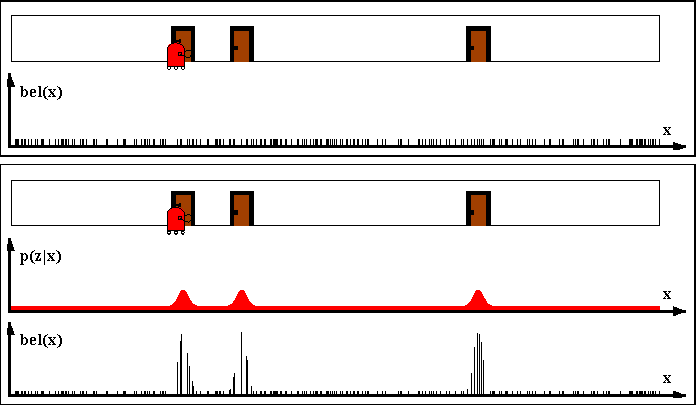
\includegraphics[width=0.8\textwidth]{./images/particle_filter/monte_carlo_correction.pdf}
    \end{center}

\end{frame}

\begin{frame}
    \frametitle{Monte Carlo Localization - Remuestreo y Predicción}

    \begin{center}
        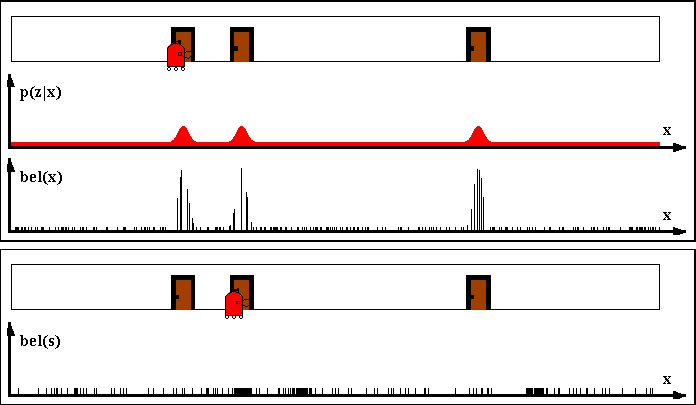
\includegraphics[width=0.8\textwidth]{./images/particle_filter/monte_carlo_resample_and_predict.pdf}
    \end{center}

\end{frame}

\begin{frame}
    \frametitle{Monte Carlo Localization - Paso de Corrección 2}

    \begin{center}
        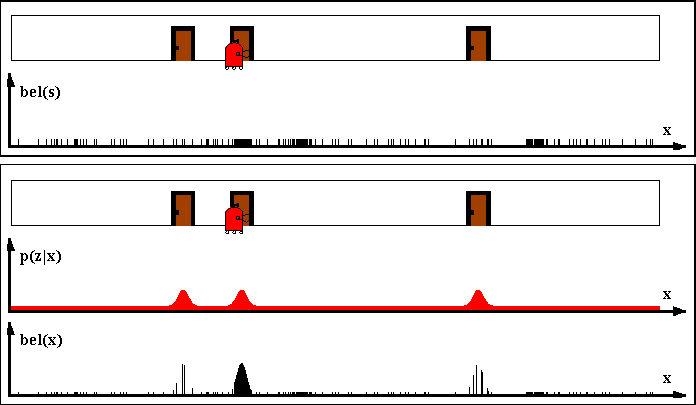
\includegraphics[width=0.8\textwidth]{./images/particle_filter/monte_carlo_correction2.pdf}
    \end{center}

\end{frame}

\begin{frame}
    \frametitle{Monte Carlo Localization - Remuestreo y Predicción 2}

    \begin{center}
        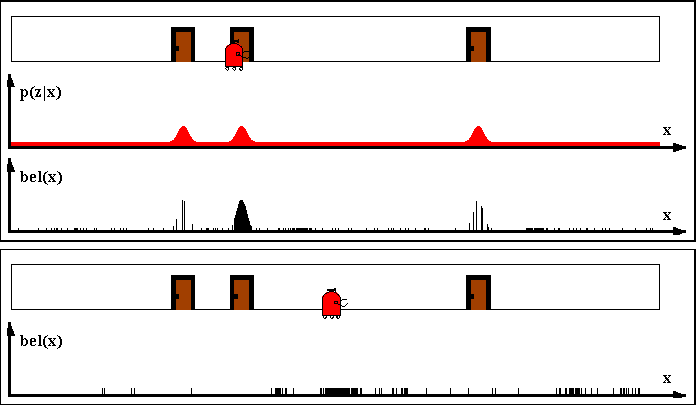
\includegraphics[width=0.8\textwidth]{./images/particle_filter/monte_carlo_resample_and_predict2.pdf}
    \end{center}

\end{frame}


\begin{frame}
    \frametitle{Resampling}
    \begin{itemize}
        \item La supervivencia del más apto: “Reemplazar muestras improbables por otras más probables”
        \item “Truco” para evitar que muchas muestras cubran estados improbables
        \item Necesario, ya que tenemos un número limitado de muestras
    \end{itemize}
\end{frame}
    
\begin{frame}
    \frametitle{Resampling Methods}
    \begin{itemize}
        \item Ruleta
        \item Búsqueda binaria (O(n log n))
        \item Muestreo universal estocástico (baja varianza, O(n))
    \end{itemize}
\end{frame}
    
\begin{frame}
    \frametitle{Low Variance Resampling}
    \begin{algorithmic}[1]
    \State $\bar{\mathcal{X}}_t = \emptyset$
    \State $r = \text{rand}(0; M^{-1})$
    \State $c = w_t^{[1]}$
    \State $i = 1$
    \For{$m = 1$ to $M$}
        \State $U = r + (m - 1) \cdot M^{-1}$
        \While{$U > c$}
            \State $i = i + 1$
            \State $c = c + w_t^{[i]}$
        \EndWhile
        \State Add $x_t^{[i]}$ to $\bar{\mathcal{X}}_t$
    \EndFor
    \State Return $\bar{\mathcal{X}}_t$
    \end{algorithmic}
\end{frame}
    
\begin{frame}
    \frametitle{Summary – Particle Filters}
    \begin{itemize}
        \item Particle filters are non-parametric, recursive Bayes filters
        \item Posterior is represented by a set of weighted samples
        \item Not limited to Gaussians
        \item Proposal to draw new samples
        \item Weight to account for the differences between the proposal and the target
        \item Work well in low-dimensional spaces
    \end{itemize}
\end{frame}
    
\begin{frame}
    \frametitle{Summary – PF Localization}
    \begin{itemize}
        \item Particles are propagated according to the motion model
        \item They are weighted according to the likelihood of the observation
        \item Called: Monte-Carlo localization (MCL)
        \item MCL is the gold standard for mobile robot localization today
    \end{itemize}
\end{frame}



\begin{frame}
    \frametitle{Material para Particle Filter}
    
    \begin{itemize}
        \item Información extraída de Vídeo de Cyrill Stachniss https://youtu.be/MsYlueVDLI0
        \item https://rse-lab.cs.washington.edu/projects/mcl/
        \item http://ais.informatik.uni-freiburg.de/teaching/ws12/mapping/pdf/slam09-particle-filter.pdf
    \end{itemize}
   
\end{frame}


\begin{frame}
    \frametitle{TODO}
    \note{Información extraída de Vídeo de Cyrill Stachniss https://youtu.be/MsYlueVDLI0}
    \note{https://rse-lab.cs.washington.edu/projects/mcl/}
    
    \TODO{UTILIZAR LAS SLIDES DEL SEMINARIO}
    
    
\end{frame}


    

	
	\section{Bibliografía}
	\begin{frame}
	\frametitle{Bibliografía}
	
	Capítulo 3 y 7 de: \cite{thrun2005probabilistic}
	
	Shon and Lindsen: Manipulating the Multivariate Gaussian Density
	
	\printbibliography
	
\end{frame}
	
	% Programming a robotic car seminar slides
	%\section{Medición}

\begin{frame}{Belief luego de sensar}
    \begin{block}{Ejemplo}
        \begin{itemize}
            \item Un mundo constituido por cinco celdas $x_{i}$ donde $i = 1, \dots ,5$
            \item Las celdas $x_{2}$ y $x_{3}$ son rojas, y el resto verdes.
            \item Inicialmente el robot desconoce su posición
            \item La probabilidad de que el robot sense correctamente  esta dada por la siguiente distribución de probabilidades:
            
            \begin{displaymath}
                P(sensa \ color | x_{i} = color) = 0.6
            \end{displaymath}
            \begin{displaymath}
                P(sensa \ \neg color | x_{i} = color) = 0.2
            \end{displaymath}
            
            Observar que no es una distribución de probabilidad correcta ya que la suma debe ser $1$.
            
        \end{itemize}
        
    \end{block}
    
    \begin{center}
        \includegraphics<1>[height=1.0cm]{./images/uniform_five_cells.png}
    \end{center}
    
\end{frame}

\begin{frame}{Belief luego de sensar}
    
    Si el robot \alert{sensa rojo}, ?`Cuál es su Posterior belief?
    
    \begin{center}
        \includegraphics<1>[height=3.5cm]{./images/inaccurate_sensing_quiz.png}
    \end{center}
\end{frame}

\begin{frame}{Belief luego de sensar}
    
    Si el robot \alert{sensa rojo}, ?`Cuál es su Posterior belief?
    
    \begin{center}
        \includegraphics<1>[height=3.5cm]{./images/inaccurate_sensing_solution.png}
    \end{center}
    \begin{footnotesize}
        \begin{displaymath}
            P(x_{i} = rojo | sensa \ rojo) = P(sensa \ rojo | x_{i} = rojo) P(x_{i}) = 0.2 \times 0.6 = 0.12
        \end{displaymath}
        \begin{displaymath}
            P(x_{i} = verde | sensa \ rojo) = P(sensa \ rojo | x_{i} = verde) P(x_{i}) = 0.2 \times 0.2 = 0.04
        \end{displaymath}
    \end{footnotesize}
    
\end{frame}

\begin{frame}{Belief luego de sensar}
    \begin{displaymath}
        P(x_{i} = rojo | sensa \ rojo) = 0.12
    \end{displaymath}
    \begin{displaymath}
        P(x_{i} = verde | sensa \ rojo) = 0.04
    \end{displaymath}
    
    Observar que estamos ante una distribución de probabilidades formalmente incorrecta dado que la suma: 
    \begin{displaymath}
        \sum_{i=1}^{5} P(x_{i}) = 0.04 + 0.12 + 0.12 + 0.04 + 0.04 = 0.36
    \end{displaymath}
    
    
    Si normalizamos la distribución, queda:
    
    \begin{displaymath}
        P(x_{i} = rojo| sensa \ rojo) = \dfrac{0.12}{0.36} = \dfrac{1}{3}
    \end{displaymath}
    \begin{displaymath}
        P(x_{i} = verde| sensa \ rojo) = \dfrac{0.04}{0.36} = \dfrac{1}{9}
    \end{displaymath}
    
    En general, $P(x_{i}|z)$ es la distribución Posterior belief del lugar $x_{i}$ dada la medición $z$.
\end{frame}


\begin{frame}{Regla de Bayes}
    
    Notar que cuando el robot sensa no hace otra cosa que aplicar la Regla Bayes:
    
    \begin{block}{Regla de Bayes}
        \begin{displaymath}
            P(x_{i} | z) = \dfrac{P(z | x_{i})P(x_{i})} {P(z)} 
        \end{displaymath}
        $P(x_{i} | z)$ : probabilidad a Posteriori (Posterior Belief) \\
        $P(z | x_{i})$ : probabilidad de Medición \\
        $P(x_{i})$ : probabilidad a Priori \\
        $P(z)$ : término de Normalización
    \end{block}
    
\end{frame}

\section{Motricidad}
\begin{frame}{Belief luego del movimiento}
    \begin{block}{Ejemplo (continuación)}
        \begin{itemize}
            \item Un mundo \alert{cíclico} constituido por cinco celdas $x_{i}$ donde $i = 1, \dots ,5$
            \item La distribución de probabilidad a priori esta determinada por:
            \begin{displaymath}
                P(x_{1}) = P(x_{4}) = P(x_{5}) = \dfrac{1}{9}
            \end{displaymath}
            \begin{displaymath}
                P(x_{2}) = P(x_{3}) = \dfrac{1}{3}    
            \end{displaymath}
        \end{itemize}
    \end{block}
    
\end{frame}

\begin{frame}{Belief luego del movimiento}
    Si el robot tiene una \alert{motricidad exacta} y desea moverse \alert{una} celda a la derecha, ?`Cuál es su Posterior belief?
    
    \begin{center}
        \includegraphics<1>[height=3.5cm]{./images/exact_motion_quiz.png}
    \end{center}
    
\end{frame}

\begin{frame}{Belief luego del movimiento}
    Si el robot tiene una \alert{motricidad exacta} y desea moverse \alert{una} celda a la derecha, ?`Cuál es su Posterior belief?
    
    \begin{center}
        \includegraphics<1>[height=3.5cm]{./images/exact_motion_solution.png}
    \end{center}
    
\end{frame}

\begin{frame}{Belief luego del movimiento}
    Suponiendo ahora que el robot desea moverse \alert{dos} celdas a la derecha y tiene una \alert{motricidad inexacta} con la siguiente distribución de probabilidad:
    \begin{columns}[t]
        \begin{column}{5cm}
            \begin{displaymath}
                P(x_{i+2}| x_{i}) = 0.8
            \end{displaymath}
            \begin{displaymath}
                P(x_{i+1}| x_{i}) = 0.1
            \end{displaymath}
            \begin{displaymath}
                P(x_{i+3}| x_{i}) = 0.1
            \end{displaymath}
        \end{column}
        \begin{column}{5cm}
            \begin{center}
                \includegraphics<1>[height=1.8cm]{./images/inexact_motion.png}
            \end{center}
        \end{column}
    \end{columns}
\end{frame}

\begin{frame}{Belief luego del movimiento}
    
    Si el robot conoce exactamente cuál es su posición inicial, ?`Cuál es su Posterior belief?
    
    \begin{columns}[t]
        \begin{column}{5cm}
            \begin{center}
                \includegraphics<1>[height=2.0cm]            {./images/inexact_motion_initial_pose_quiz.png}
            \end{center}
        \end{column}
        \begin{column}{5cm}
            \begin{center}
                \includegraphics<1>[height=1.8cm]{./images/inexact_motion.png}
            \end{center}
        \end{column}
    \end{columns}
\end{frame}

\begin{frame}{Belief luego del movimiento}
    
    Si el robot conoce exactamente cuál es su posición inicial, ?`Cuál es su Posterior belief?
    
    \begin{columns}[t]
        \begin{column}{5cm}
            \begin{center}
                \includegraphics<1>[height=2cm]            {./images/inexact_motion_initial_pose_solution.png}
            \end{center}
        \end{column}
        \begin{column}{5cm}
            \begin{center}
                \includegraphics<1>[height=1.8cm]{./images/inexact_motion.png}
            \end{center}
        \end{column}
    \end{columns}
\end{frame}

\begin{frame}{Belief luego del movimiento}
    Si el robot tiene como distribución inicial que se encuentra en las celdas $x_{2}$ y $x_{4}$ con igual probabilidad, formalmente,
    \begin{displaymath}
        P(x_{2}) = P(x_{4}) = 0.5
    \end{displaymath}
    ?`Cuál es su Posterior belief?
    
    \begin{columns}[t]
        \begin{column}{5cm}
            \begin{center}
                \includegraphics<1>[height=2cm]{./images/inexact_motion_quiz.png}
            \end{center}
        \end{column}
        \begin{column}{5cm}
            \begin{center}
                \includegraphics<1>[height=1.8cm]{./images/inexact_motion.png}
            \end{center}
        \end{column}
    \end{columns}
\end{frame}

\begin{frame}{Belief luego del movimiento}
    
    Si el robot tiene como distribución inicial que se encuentra en las celdas $x_{2}$ y $x_{4}$ con igual probabilidad, formalmente,
    \begin{displaymath}
        P(x_{2}) = P(x_{4}) = 0.5
    \end{displaymath}
    ?`Cuál es su Posterior belief?
    
    \begin{columns}[t]
        \begin{column}{5cm}
            \begin{center}
                \includegraphics<1>[height=2cm]{./images/inexact_motion_solution.png}
            \end{center}
        \end{column}
        \begin{column}{5cm}
            \begin{center}
                \includegraphics<1>[height=1.8cm]{./images/inexact_motion.png}
            \end{center}
        \end{column}
    \end{columns}
    \begin{small}
        $P(x_{1}) = P(x_{4}) P(x_{1}|x_{4}) = 0.5 \times 0.8 = 0.4$ \\
        $P(x_{2}) = P(x_{4}) P(x_{2}|x_{4}) = 0.5 \times 0.1 = 0.05$ \\
        $P(x_{3}) = P(x_{2}) P(x_{3}|x_{2}) = 0.5 \times 0.1 = 0.05$ \\    
        $P(x_{4}) = P(x_{2}) P(x_{4}|x_{2}) = 0.5 \times 0.8 = 0.4$ \\    
        $P(x_{5}) = P(x_{2}) {\color{red} P(x_{5}|x_{2})} + P(x_{4}) {\color{green} P(x_{5}|x_{4})} = 0.5 \times {\color{red} 0.1} + 0.5 \times {\color{green} 0.1} = 0.1$    
    \end{small}
\end{frame}

\section{Sensar y Mover}
\begin{frame}{Ciclo de sensar y mover}
    Localización no es más que la iteración de sensar y mover.
    \begin{center}
        \includegraphics<1>[height=2.5cm]{./images/sens_and_move.pdf}
    \end{center}
    
    \begin{block}{Entropía}
        Medida de información que tiene la distribución
        \begin{displaymath}
            - \sum P(x_{i}) \log P(x_{i})
        \end{displaymath}
        
        En otras palabras, la entropía expresa la información que un robot recibe luego de ejecutar una acción específica.
    \end{block}
    
\end{frame}


\begin{frame}{Definición formal de localización}
    
    \begin{block}{Medición}
        \begin{displaymath}
            \Bar{P}(x_{i}|z) \leftarrow P(z|x_{i}) P(x_{i})
        \end{displaymath}
        \begin{displaymath}
            \alpha \leftarrow \sum \Bar{P}(x_{i}|z)
        \end{displaymath}
        \begin{displaymath}
            P(x_{i}|z) \leftarrow \frac{1}{\alpha} \Bar{P}(x_{i}|z)
        \end{displaymath}
        
    \end{block}
    
\end{frame}

\begin{frame}{Definición formal de localización}
    
    Sea $P(x_{i}^{t})$ la probabilidad de estar en el punto $x_{i}$ luego del movimiento del robot
    
    \begin{block}{Motricidad}
        
        \begin{displaymath}
            P(x_{i}^{t}) = \sum_{j} P(x_{j}^{t-1}) P(x_{i}|x_{j})
        \end{displaymath}
        
    \end{block}
    
    La probabilidad de estar en $x_{i}$ se calcula a través de todos los lugares de los que podríamos haber venido
    
    Observar que la expresión anterior no es otra cosa que el Teorema de Probabilidad total.
    
    \begin{block}{Teorema de Probabilidad Total}
        
        \begin{displaymath}
            P(A) = \sum_{B}^{}P(A|B) P(B)
        \end{displaymath}
        
    \end{block}
    
\end{frame}
	
\end{document}